\documentclass[12pt,fleqn]{article}\usepackage{../../common}
\begin{document}
Değişim Noktası Analizi (Changepoint Analysis)

İngiltere'de 1851 ve 1962 yılları arasında kömür madenlerinde olan
kazaların sayısı yıllık olarak kayıtlıdır. Acaba bu kazaların dağılımına
bakarak, değişimin olduğu seneyi bulabilir miyiz? Böyle bir değişim anı
neyi gösterir? Belki madenlerle alakalı regülasyonlarda, denetimlerde bir
değişiklik olmuştur, ve kaza oranı azalmıştır [1, 2], [3, sf. 141]. Veriye
bakalım.

\begin{minted}[fontsize=\footnotesize]{python}
import pandas as pd
coal = pd.read_csv('coal.txt',header=None)
\end{minted}

\begin{minted}[fontsize=\footnotesize]{python}
coal.hist(bins=7)
plt.savefig('stat_coal_02.png')
\end{minted}

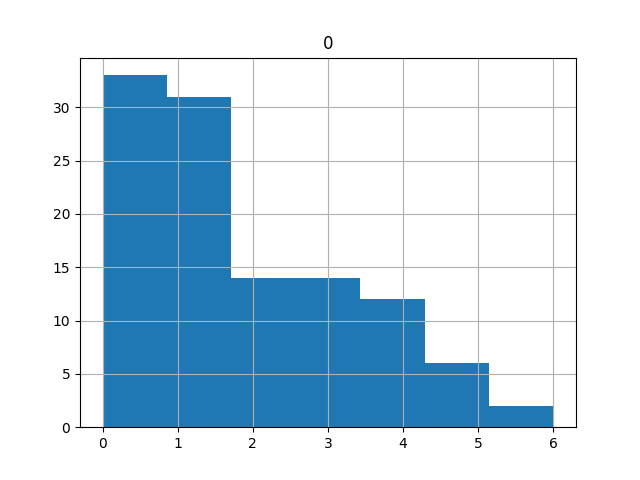
\includegraphics[height=6cm]{stat_coal_02.png}

Eğer veride bir değişim noktası var ise, bu durum veride iki fark bölge
olduğunu gösterir, ki bu bölgelerin iki farklı dağılımla temsil edileceğini
tahmin edebiliriz. 

Aynı zaman diliminde vuku bulan olay toplamlarının (event counts) Poisson
dağılımına sahip olduğunu biliyoruz. O zaman, belki de ilk yapmamız gereken
bu veriye iki tane Poisson uydurmak, yani veriyi iki Poisson dağılımının
karışımı olarak temsil etmek. Karışımlar konusu [5] yazısında görülebilir,
buradaki tek fark Bernoulli yerine Poisson kullanılacak olması. İdeal
olarak uydurma operasyonu için Beklenti-Maksimizasyon
(Expectation-Maximization -EM-) kullanılır. Fakat denklemleri türetmek
zaman alabilir, biz şuradaki tavsiyeyi [4, sf. 11] takip ederek bu örnek
için uydurmayı bir gayrı lineer optimizasyon paketi \verb!lmfit! ile
yapacağız (tavsiyenin R kodu \verb!coal.r! içinde).

\begin{minted}[fontsize=\footnotesize]{python}
from scipy.stats.distributions import poisson
from lmfit import Parameters, minimize
from lmfit.printfuncs import report_fit

def f(pars,x):
    m1 = pars['m1'].value
    lam1 = pars['lam1'].value
    lam2 = pars['lam2'].value
    model = m1*poisson(lam1).pmf(x) + (1-m1)*poisson(lam2).pmf(x) 
    return model
    
def residual(pars,y,x):
    return -np.log(f(pars,x).T[0])

fit_params = Parameters()
fit_params.add('m1', value=0.5, min=0,max=1.)
fit_params.add('lam1', value=1.0, min=1.,max=7.)
fit_params.add('lam2', value=2.0, min=2.,max=7.)

out = minimize(residual, fit_params, args=(coal,coal,))
report_fit(fit_params)
\end{minted}

\begin{verbatim}
[[Variables]]
    m1:     0.51428096 +/- 0.406949 (79.13%) (init= 0.5)
    lam1:   1.00000004 +/- 0.557045 (55.70%) (init= 1)
    lam2:   3.35150806 +/- 1.791094 (53.44%) (init= 2)
[[Correlations]] (unreported correlations are <  0.100)
    C(m1, lam1)                  =  0.905 
    C(m1, lam2)                  =  0.878 
    C(lam1, lam2)                =  0.772 
\end{verbatim}

Sonuçlar yaklaşık $\lambda_1=1,\lambda_2=3$ (tam sayıya yuvarladık, çünkü
olay sayısı tam sayı olmalı). Bu iki dağılımı verinini normalize
edilmiş histogramı üzerinde gösterirsek,

\begin{minted}[fontsize=\footnotesize]{python}
from scipy.stats.distributions import poisson
coal.hist(bins=7,normed=True)
plt.hold(True)
p = poisson(1.0)
x = np.arange(1,10)
plt.plot(x, p.pmf(x))
p = poisson(3.0)
plt.hold(True)
plt.plot(x, p.pmf(x))
plt.savefig('stat_coal_03.png')
\end{minted}

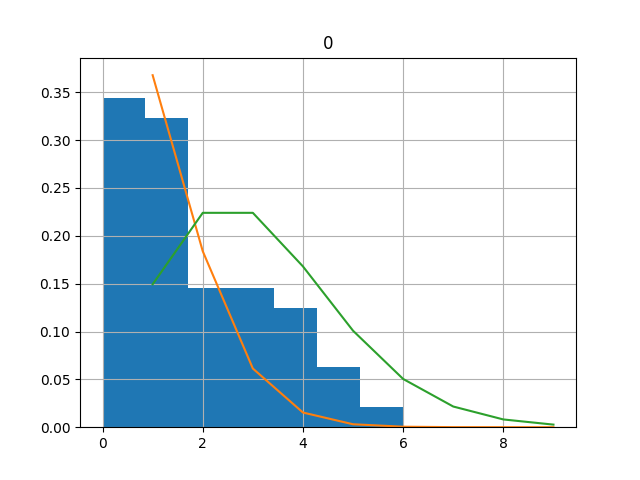
\includegraphics[height=6cm]{stat_coal_03.png}

Peki bu bulguyu şimdi değişim noktası keşfine nasıl çevireceğiz? Dikkat,
üstteki iki dağılımın ayrıldığı $\lambda$ anı değil aradığımız, verideki
senesel akış içinde hangi sene sonrası bir dağılımın diğerinin yerine
geçtiği. 

Şöyle bir yaklaşım olabilir mi acaba: bir döngü içinde potansiyel ayraç
noktası olabilecek tüm seneler için veriyi iki parçaya ayırırız. Sıfır
hipotezi nedir? Bu veri parçaları üstteki bulduğumuz Poisson
dağılımlarından geliyor. O zaman şöyle devam ederiz: Üstteki
optimizasyondan elimizde her iki dağılımın beklentisi, yani $\lambda$
değerleri var, ve Poisson dağılımlarının bir avantajı beklentisinin ve
varyansının aynı olması!  Şimdi, eğer her iki parçanın sayısal ortalamasını
ve sıfır hipoteze göre bilinen $\mu,\sigma^2$ (her ikisi de $\lambda$)
üzerinden standardize edersek, yani $N(0,1)$ haline getirirsek, elimize iki
tane $N(0,1)$ geçer, diyelim ki $Z_1,Z_2$. Bunların karelerinin toplamının
chi kare olacağını biliyoruz. Sıfır hipotezine göre böyle olmalı. O zaman
bundan ``sapma'' sıfır hipotezinden ne kadar uzaklaşıldığını gösterir, bu
bağlamda en yüksek p-değerini veren ayraç noktası bize değişim anını verir.

Daha detaylı matematiği vermek gerekirse; Merkezi Limit Teori'sine göre
birbirinden bağımsız, aynı dağılımlı $X_1,..,X_n$'in, ki her birinin
beklentisi $E(X_i) = \mu$ ve varyansı $Var(X_i)=\sigma^2$, o zaman sayısal
ortalama $\bar{X}$ üzerinden, ve $n \to \infty$

$$ Z = \frac{\bar{X} - \mu }{\sigma \sqrt{n}}   $$

yani standard normal $Z \sim N(0,1)$. Daha önce belirttiğimiz gibi Poisson
için $\mu = \sigma^2$. 

Gerekli olan diğer teori: $\chi_{n}^2 \sim Z_1^2 + ... + Z_n^2$, yani $n$
tane standart normalın toplamı yaklaşık olarak serbestlik derecesi $n$ olan
chi kare dağılımı. Bu iki bilgiyi yan yana koyarsak, ve üstte bahsettiğimiz
döngüyü yazarsak,

\begin{minted}[fontsize=\footnotesize]{python}
from scipy.stats import chi2
# buyuk olan lambda degerini ilk parca icin kullaniyoruz, cunku
# test ettigimiz kaza oranlarinin once fazla sonra az olmasi
lam1 = 3.; lam2 = 1.
dof = 2
res = []
cutoffs = range(20,80)
for cutoff in cutoffs:
     p1 = coal[0:cutoff]; p2 = coal[cutoff+1:]
     z1 = (p1.mean()-lam1) / lam1*np.sqrt(len(p1))
     z2 = (p2.mean()-lam2) / lam2*np.sqrt(len(p2))
     chi = z1**2+z2**2
     res.append(float(1-chi2.cdf(chi,dof)))

print 1851 + cutoffs[np.array(res).argmax()]
\end{minted}

\begin{verbatim}
1885
\end{verbatim}

Tarihten biliyoruz ki değişimin sebebi büyük ihtimalle İngiltere'de 1887
yılında kanunlaşan {\em Kömür Madenleri Yasası}'dır [3]. Yakınlık fena
değil.

Ödev: Verinin iki tane Poisson karışımıyla temsil edilmesi gerektiğinden
emin olmak istiyorsak, AIC kullanarak tek Poisson uyumu, daha sonra
karışımın uyumu için ayrı ayrı AIC'leri hesaplayarak hangisinin daha düşük
olduğuna göre bu kararı verebiliriz.

Bayes ve MCMC 

Bir değişik yöntem Bayes yaklaşımını kullanarak ve hesapsal olarak Markov
Chain Monte Carlo (MCMC) tekniği. Kazaların sayısının tümünü iki Poisson
dağılımının ortak dağılımı (joint distribution) üzerinden modelleyeceğiz,
ve bu dağılımların birinci Poisson'dan ikincisine geçtiği anı hesaplamaya
uğraşacağız.

Poisson dağılımı

$$ p(y|\theta) = \frac{e^{-\theta}\theta^y}{y!} $$

Eldeki n tane veri noktası $y=y_0, y_1,...,y_n$'nin hep birlikte
$\theta$ ile tanımlı bir Poisson dağılımından gelip gelmediğinin ne
kadar mümkün olduğu (likelihood) hesabı şöyledir:

$$ p(y|\theta) = \frac{e^{-n\theta}\theta^{\sum y_i}}{\prod y_i!}  $$

Formülün bölünen kısmındaki tüm y noktaları toplanıyor, bölen kısminde
ise tüm y değerleri teker teker faktoryel hesabı sonrası birbiri ile
çarpılıyor.

Şimdi yukarıdaki $\theta$ değişkeni de noktasal bir değer yerine bir
"dağılıma", mesela $\theta$ Gamma dağılımına sahip olabilirdi:
$Gamma(\alpha, \beta)$. Formülde $\alpha$, $\beta$ sabit değerlerdir
(fonksiyon değişkeni değil). Gamma olasılık formülü şöyledir:

$$ p(\theta) = \frac{\beta^\alpha}{\Gamma(\alpha)}\theta^{\alpha-1}e^{-\beta\theta} $$

O zaman $p(y|\theta)$ formülünü bulmak için Bayes teorisini
kullanmamız gerekecekti. Bayes teorisi bilindiği gibi

$$ p(\theta|y) = \frac{p(y|\theta)p(\theta)}{p(y)} $$

$$ p(\theta|y) \propto p(y|\theta)p(\theta) $$

İkinci formüle dikkat, eşitlik yerine orantılı olma (proportional to)
işaretini kullanıyor. Sebep: bölen kısmındaki p(y)'yi kaldırdık, sonuç
olarak soldaki $p(\theta|y)$ değeri artık bir dağılım değil -- bu bir
bakımdan önemli ama örnekleme amacı için bir fark yaratmıyor,
basitleştirme amacıyla bunu yaptık, böylece $p(y)$'yi hesaplamamız
gerekmeyecek, ama örnekleme üzerinden diğer tüm hesapları hala
yapabiliriz. Tamam.

Şimdi Bayes Teorisini Gamma önsel (apriori) ve Poisson olurluğu
(likelihood) üzerinden kullanırsak,

$$ 
p(\theta|y) = \frac{\beta^\alpha}{\Gamma(\alpha)}
\theta^{\alpha-1}e^{-\beta\theta} \times
\frac{e^{-n\theta}\theta^{\sum y}}{\prod y!} 
$$

Benzer terimleri yanyana getirelim:

$$ 
p(\theta|y) = \frac{\beta^\alpha}{\Gamma(\alpha)\prod y!}
\theta^{\alpha-1}\theta^{\sum y}e^{-\beta\theta} e^{-n\theta} 
$$

Şimdi sol taraftaki bölümü atalım; yine üsttekine benzer numara, bu
kısım gidince geri galan dağılım olamayacak, ama ona "oranlı" başka
bir formül olacak.

$$ p(\theta|y)  \propto  \theta^{\alpha-1}\theta^{\sum y}e^{-\beta\theta} e^{-n\theta} $$

$$  \propto \theta^{\alpha-1+\sum y}e^{-(\beta+n)\theta}  $$

Bu dağılım nedir? Formülün sağ tarafı Gamma dağılımının formülüne
benzemiyor mu?  Evet, formülün sağ tarafı $Gamma(\alpha+\sum y, \beta
+ n)$ dağılımı, yani ona orantılı olan bir formül. Yani Bayes teorisi
üzerinden şunu anlamış olduk; eğer önsel dağılım Gamma ise, Poisson
mümkünlük bizi tekrar Gamma sonuç dağılımına götürüyor. Gamma'dan
başlayınca tekrar Gamma'ya ulaşıyoruz. Bu bir rahatlık, bir kolaylık,
bir matematiksel numara olarak kullanılabilir. Sonsal (posterior)
dağılımların şekli, hesaplanma, cebirsel işlemler açısından önemli,
eğer temiz, kısa, öz olurlarsa hesap işlerimiz kolaylaşır.

Not: Hatta üzerinde çalıştığımız problem sebebiyle eğer Poisson
mümkünlük olacağını biliyorsak, sadece bu sebeple bile önsel dağılımı,
üstteki kolaylık bilindiği için, özellikle Gamma seçebiliriz, çünkü
biliriz ki Gamma ile başlarsak elimize tekrar Gamma geçecektir.

Şimdi kömür madeni verisine gelelim. Bu madendeki kazaların sayısının Poisson
dağılımından geldiğini öne sürüyoruz, ve kazaların "iki türlü" olduğunu
bildiğimizden hareketle, birinci tur kazaların ikinci tur kazalardan değişik
Poisson parametresi kullandığını öne süreceğiz.

O zaman değişim anını, değişim senesini nasıl hesaplarız?

Kazaların ilk k senede ortalama $\theta$ ile, ve k ve n arasındaki
senelerde ortalama $\lambda$ Poisson ile dağıldığını söyleyelim: Yani

$$ Y_i = Poisson(\theta) \qquad i=1,..,k   $$

$$ Y_i = Poisson(\lambda) \qquad i=k+1,..,n $$

Burada $Y_i$ sene i sırasında olan kazaların sayısını belirtiyor. Bayes kuralını
hatırlarsak $\theta$ ve $\lambda$ parametrelerine önsel dağılım atayacağız. Bu
dağılım Gamma olacak. Yani $\theta \sim Gamma(a_1, b_1)$ ve $\lambda \sim
Gamma(a_2, b_2)$.

Ayrıca k değerini de bilmiyoruz, k değeri yani "değişim noktası" Poisson
dağılımların birinden ötekine geçtiği andır. Bu seneyi bulmaya
çalışıyoruz. Şimdi tüm verinin, tüm seneleri kapsayacak şekilde modelini
kurmaya başlayalım. k parametresinin aynen öteki parametreler gibi bir
önsel dağılımı olacak (ki sonradan elimize k için de bir sonsal dağılımı
geçecek), ama bu parametre elimizdeki 112 senenin herhangi birinde "eşit
olasılıkta" olabileceği için onun önsel dağılımı Gamma değil $k \sim Unif(1,112)$ 
olacak. Yani ilk başta her senenin olasılığı birbiriyle eşit,
her sene $\frac{1}{112}$ olasılık değeri taşıyor.

Bu modelin tamamının olurluğu nedir?

$$ L(\theta, \lambda, k | y) = \frac{1}{112} \times \displaystyle \prod_{i=1}^k
\frac{e^{-\theta}\theta^{y_i}}{y_i!}  \times \displaystyle \prod_{i=k+1}^n
\frac{e^{-\lambda}\lambda^{y_i}}{y_i!} 
 $$

Sonsal geçişini yapınca yukarıda olduğu gibi Gamma dağılımlarını elde
ederiz:

$$ L(\theta, \lambda, k | y)  \propto 
\theta^{a_1-1+\sum_{i=1}^{k} y_i}e^{-(b_1+k)\theta} 
\lambda^{a_2-1+\sum_{i=k+1}^n y_i}e^{-(b_2+n-k)\lambda} 
 $$

$\frac{1}{112}$'yi bir sabit olduğu için formülden attık, bu durum orantılı hali
etkilemiyor. Üstteki formül içindeki Gamma dağılımlarını görebiliyoruz, hemen
yerlerine koyalım:

$$ L(\theta, \lambda, k | y)  \propto 
Gamma(a_1 + \sum_{i=1}^{k} y_i, b_1+k) \
Gamma(a_2 + \sum_{i=k+1}^{n} y_i, b_2+n-k)
 $$

Gibbs örneklemeye gelelim. Bu örneklemeye göre şartsal dağılım (conditional
distribution) formülü bulunmaya uğraşılır, hangi değişkenlerin verili olduğuna
göre, o değişkenler sabit kabul edilebilir, ve orantısal formülden
atılabilir. Bu her değişken için teker teker yapılır. 

Sonra hesap sırasında her şartsal dağılıma teker teker zar attırılır, ve
elde edilen değer, bu sefer diğer şartsal dağılımlara değer olarak
geçilir. Bu işlem sonuca erişilinceye kadar özyineli (iterative) olarak
tekrar edilir (mesela 1000 kere). O zaman,

$$ \theta | Y_1,..,Y_n,k \sim Gamma(a_1 + \sum_{i=1}^{k} y_i, b_1+k) $$

$$ \lambda | Y_1,..,Y_n,k \sim Gamma(a_2 + \sum_{i=k+1}^{n} y_i, b_2+n-k) $$

$$ 
p(k | Y_1,..,Y_n) \propto \theta^{\sum_{i=1}^{k} y_i}e^{-k\theta} 
\lambda^{\sum_{i=k+1}^n y_i}e^{k\lambda} 
 $$

En son formülde içinde k olan terimleri tuttuk, gerisini attık. Formül $e$
terimleri birleştirilerek biraz daha basitleştirilebilir:

$$ p(k | Y_1,..,Y_n) \propto
\theta^{\sum_{i=1}^{k} y_i} \lambda^{\sum_{i=k+1}^n y_i}e^{(\lambda-\theta)k} 
 $$

Bir basitleştirme daha şöyle olabilir

$$ K = \sum_{i=1}^{k} y_i  $$

$$ \lambda^{\sum_{i=k+1}^n y_i} = \lambda^{\sum_{i=1}^n y_i - \sum_{i=1}^k y_i} $$

Üstel işlemlerde eksi işareti, üstel değişken ayrılınca bölüm işlemine dönüşür:

$$ = \frac{\lambda^{\sum_{i=1}^n y_i}}{\lambda ^{\sum_{i=1}^k y_i}} $$

$$ = \frac{\lambda^{\sum_{i=1}^n y_i}}{\lambda ^{K}} $$

$$ p(k | Y_1,..,Y_n) \propto 
\theta^{K} \frac{\lambda^{\sum_{i=1}^n y_i}}{\lambda ^{K}} e^{(\lambda-\theta)k} 
 $$

$$ = \bigg(\frac{\theta}{\lambda}\bigg)^{K} \lambda^{\sum_{i=1}^n  y_i} e^{(\lambda-\theta)k} $$

$\lambda^{\sum_{i=1}^n y_i}$ terimi $k$'ye değil $n$'ye bağlı olduğu
için o da final formülden atılabilir

$$  
p(k | Y_1,..,Y_n) \propto \bigg(\frac{\theta}{\lambda}\bigg)^{K} 
e^{(\lambda-\theta)k}  
$$  

$p(k)$ için ortaya çıkan bu formüle bakarsak, elimizde verilen her k
değeri için bir olasılık döndürecek bir formül var. Daha önceki Gamma
örneğinde formüle bakarak elimizde hemen bir Gamma dağılımı olduğunu
söyleyebilmiştik. Bu kodlama sırasında işimize yarayacak bir şeydi,
hesaplama için bir dağılıma "zar attırmamız" gerekiyor, ve Gamma
örneğinde hemen Python Numpy kütüphanesindeki random.gamma çağrısına
Gamma'dan gelen rasgele sayılar ürettirebiliriz. Üstteki formüle
bakarsak, hangi dağılıma zar attıracağız?

Cevap şöyle: $p(k|..)$ pdf fonsiyonundaki k değişkeni $1,..,119$ arasındaki
tam sayı değerleri alabilir, o zaman ortada bir ayrıksal (discrete) dağılım
var demektir. Ve her k noktası için olabilecek olasılık değerini üstteki
$p(k|..)$ formülüne hesaplattırabiliyorsak, ayrıksal bir dağılımı her nokta
için üstteki çağrı, ve bu sonuçları normalize ederek (vektörün her
elemanını vektörün toplamına bölerek) bir dağılım şekline
dönüştürebiliriz. Daha sonra bu "vektörsel dağılım" üzerinden zar
attırırız. Python kodundaki \verb!w_choice! ya da R dilindeki \verb!sample!
çağrısı bu işi yapar.

\begin{minted}[fontsize=\footnotesize]{python}
import math
import random

np.random.seed(0); random.seed(0)

# samples indexes from a sequence of probability table
# based on those probabilities
def w_choice(lst):
    n = random.uniform(0, 1)
    for item, weight in enumerate(lst):
        if n < weight:
            break
        n = n - weight
    return item

#
# hyperparameters: a1, a2, b1, b2
#
def coal(n,x,init,a1,a2,b1,b2):
    nn=len(x)
    theta=init[0]
    lam=init[1]
    k = init[2]
    z=np.zeros((nn,))
    for i in range(n):
        ca = a1 + sum(x[0:k])
        theta = np.random.gamma(ca, 1/float(k + b1), 1) 
        ca = a2 + sum(x[(k+1):nn])
        lam = np.random.gamma(ca, 1/float(nn-k + b2), 1)
        for j in range(nn):
            z[j]=math.exp((lam-theta)*(j+1)) * (theta/lam)**sum(x[0:j])
        # sample
        zz = z / sum(z)
        k = w_choice(zz)
    print float(theta), float(lam), float(k)
                
data = np.loadtxt("coal.txt")
coal(1100, data, init=[1,1,30], a1=1,a2=1,b1=1,b2=1)
\end{minted}

\begin{verbatim}
3.32561369453 0.931821137936 42.0
\end{verbatim}

Kodları işletince elimize k = 42 değeri geçecek, yani değişim anı 1851+42 = 1893
senesidir. [7] kaynağına göre 1908 senesindeki Britanya kömür madenleri
regülasyonunu ilerleten kanun sayesinde kazalarda azalma olduğu zaten
söylenmektedir, demek ki gerçek değere yaklaştık.

Kaynaklar: 

[1] Ioana A. Cosma, Ludger Evers, {\em Markov Chain Monte Carlo Methods (Lecture)}

[2] Koop, {\em Bayesian Econometric Methods}

[3] Anderson, A. (1911). Labour legislation. In H. Chisholm (Ed.),
{\em Encyclopedia britannica (11th ed., Vol. 16, sf. 7-28)}

[4] Zuccini, {\em Hidden Markov Models for Time Series An Introduction Using R}

[5] Bayramli, Istatistik, {\em Çok Değişkenli Bernoulli Karışımı}

[6] {\em Bayesian estimation of changepoints},
    \url{https://ruivieira.dev/bayesian-estimation-of-changepoints.html}

[7] {\em Coal Mines Regulation Act 1908},
    \url{https://schoolshistory.org.uk/topics/british-history/modern-britain/liberal-reforms/mines-act-1908}

\end{document}
